\chapter{Markov Chains}

\section{Introduction}
A markov process is a process $X_n \text{ or } X_t$ s.t.
\begin{equation}
	\prob[X_{n+1} = j | X_0 = i_0, X_1 = i_1, \dots, X_n = i_n] = \prob[X_{n+1} = j | X_n=i_n] = P
\end{equation}

with P as the \textit{one-step probability}. From now on, the notation for that probability will be $P_{i,j}^{n,n+1}=P_{i,j} \quad \forall n$ if the MC is homogeneous, i.e. the transition probabilities are stationary.

We can suppose $n\ge 0$ and we'll have the \textbf{transition probability matrix}, which will characterize the process as
\begin{equation} \bm P=\begin{pmatrix}
	P_{00} & P_{01} & \cdots  \\
	P_{10} & P_{11} & \cdots \\
	\vdots & \vdots & \ddots  \\
 	\end{pmatrix}
	\text{with } P_{i,j}\ge 0 \forall i,j \quad \text{ and } \sum\limits_{j=0}^{+\infty}P_{i,j} = 1 \quad \forall i
\end{equation}

For example
\begin{equation}
	\prob[X_3 = i_3 , X_2 = i_2, X_1 = i_1, X_0 = i_0]=P_{i_0}\cdot P_{i_0,i_1}\cdot P_{i_1,i_2}\cdot P_{i_2,i_3}
\end{equation}

The description of a markov process is given from the initial state probability and the transition probability matrix.

\section{Stability of a process}
Suppose a system where customers arrive independently and are queued in the system before getting served.
Suppose the service time occupies only one slot and all the slots for service time have same duration.
If the queue is empty, that time slot is wasted.
Now let the number of users arriving in the n-th slot be $\xi_n$ and the number of users in
the system in the n-th slot  be $X_n$. Then we have:
 \begin{equation}
 	\begin{split}
 	&\prob[\xi_n=k] = a_k \text{, probability of k arriving users at time n}\\
  	&X_{n+1}=
		\begin{cases}
 			X_n -1 +\xi_n &  \text{if } X_n >0 \\
 			\xi_n 			 	&  \text{if } X_n = 0
 		\end{cases}
 	\end{split}
 \end{equation}

The transition probability matrix:
\begin{equation} \bm P=\begin{pmatrix}
	a_{0} & a_{1} & a_2 & \cdots  \\
	a_{0} & a_{1} & a_2 & \cdots  \\
	0			& a_{0} & a_{1} & \cdots  \\
	0 		& 0			& a_{0} & \cdots  \\
	\vdots & \vdots & \vdots & \ddots &  \\
\end{pmatrix}
\end{equation}
\begin{definition}[Behavior of a MC]
Let $\rho=\sum\limits_{k=0}^{+\infty} k \cdot a_k$. We say that for
\begin{equation} \rho : \begin{cases}
	>1 & \text{\textbf{unstable }: the system will never be able to serve everybody}\\
	=1 & \text{\textbf{unstable \textit{unless deterministic}}: sooner or later the system will fail}\\
	<1 & \text{\textbf{stable}: the queue tends to be empty}
\end{cases}\end{equation}
\end{definition}

\section{First step analysis}
\begin{definition}[Absorbent state]
	 A state $i$ is defined $absorbient$ if it is valid the following condition:$p_{ij}=0$ $\forall j\neq i$ and $p_{ii}=1$. In practice, when a chain incur in the state $i$ no transition to other different states is longer possible. Therefore  the chain will remain "absorbed" in it. 
\end{definition}
\begin{definition}[Absorbent time]
	Being $A$ the set of the absorbent states of a particular markov chain, the absorbent time is defined in the following way: 
	\begin{equation}
	T= \min \{n\geq0: X_n \in A \}
	\end{equation}
\end{definition}
"First step analysis" is a "standard procedure" applied to resolve some particular Markov Chain in which there is one of more absorbent state.
 We are interested in computing two fundamental quantities:
\begin{itemize}
	\item The probability of absorption given a starting point $i$ :  $ u_i=P[X_T\in A | X_0=i ]$
	\item The expected absorption time given a starting point $i$ : $v_i= E[T|X_0=i]$
\end{itemize}
\subsection{First Step Analysis: General Method}
\begin{itemize}
	\item Reorganize the markov chain according to the following rules
	\begin{itemize}
		\item The states from $0,..r-1$ transient;
		\item The states from $r,...,N$ absorbent.
	\end{itemize}

	\item  Reorganize the transition matrix according to the following rules :
     \begin{equation} P=\begin{pmatrix}
     P_{00} & P_{01} & \cdots & P_{0r}& P_{0(r+1)} &\cdots & \cdots &P_{0N} \\
     P_{00} & P_{01} & \cdots & P_{1r}& P_{1(r+1)}& \cdots & \cdots & P_{1N}\\
     \vdots & \vdots & \ddots  \\
     P_{r0}=0 & P_{r1}=0& \cdots &P_{rr}=1& 0 & \cdots & \cdots &0\\
     P_{(r+1)0}=0 & P_{(r+1)1}=0& \cdots &P_{(r+1)r}=0& P_{(r+1)(r+1)}=1& 0&  \cdots&  0\\
     \vdots & \vdots & \ddots  \\
     P_{N0}=0 & P_{N1}=0& \cdots &P_{Nr}=0& P_{N(r+1)}=0& 0&  \cdots&  P_{NN}=1\\
     
     \end{pmatrix}
$$   
     \end{equation}
     As shown in the figure above the matrix is composed by three parts:
     \begin{itemize}
     	\item In the upper part there are the transitions probability from the not-absorbient states.
     	\item In the low left corner there are the transition probability from  the absorbent states to the not-absorbent states: these can be have only 0 for the definition of absorbent state.
     	\item In the low-right corner there are the transition probabilities from  the absorbent states to the absorbent states. This is a $(N-r)$ x$(N-r)$ identity submatrix: once a chain enters in one absorbent state, it can only remain in it and cannot go away 
     	
     \end{itemize} 
    \item In order to compute the the probability of absorption given a starting point $i$ it is possible to write the following:
    \begin{equation} 
    \begin{split}
      u_{ik} = P[X_T=k|X_0=i]= \sum\limits_{j=0}^N u_{jk}P_{ij}=\\
      \sum\limits_{j=0}^N P[X_T=k|X_0=i,X_1=j]P[X_1=j|X_0=i]=\\
      = P_{ik}+\sum\limits_{j=0}^N 0*P_{ij} +\sum\limits_{j=0}^{r-1} u_{jk}P_{ij},
      \\
      P_{ik}+\sum\limits_{j=0}^{r-1} u_{jk}P_{ij}              
      \end{split}      
     \end{equation}
     
       this is valid for $i= 0,1,..r-1$
    Intuitively the probability of being absorbed in a state $k$ starting in $i$ is equal to the transient probability of the transition $i\rightarrow k$ plus the probabilities of being absorbent from another not-absorbent state ($j \in (0,...r-1)$) weighted by the probability of doing the transition  $i\rightarrow j$ ($P_{ij}$). 
    In this case the unknown values are the $u_{jk}$ thus 
    a system of $ r-1$ has to be solved in order to compute properly $u_{ik}$ probability.
     \newline Trivially for $i= r,.. , N$, $u_{ik}=0$ for $i\neq k$ and $u_{ik}=1$ $i=k$.
 
 \item In order to compute the expected absorption time given a starting point $i$ : $v_i= E[T|X_0=i]$ a very similar method is applied: 
 \begin{equation}
 v_i= 1 + \sum\limits_{j=0}^{r-1} P_{ij} v_j
  \end{equation}
   Intuitively the expected absorption time from i is equal to 1 with probability 1 (at least one transition has to be done) plus the  the expected absorption time starting from j weighted by the probability of doing the transition  $i\rightarrow j$ ($P_{ij}$) where j (of course) is a not-absorbent state.
   
  \item Remember that all the equations written above are recursive because they will have the following form :
  \begin{equation}
     u_{ik}= P_{ik}+\sum\limits_{j=0}^{r-1} u_{jk}P_{ij} =  P_{ik}+ u_{0k}P_{i0} + .... + u_{ik}P_{ii} + ... +  u_{(r-1)k}P_{i(r-1)}
   \end{equation}  
\end{itemize}

%\subsection{First passage time}
%Another application of first step analysis is the computation of so-called "First-passage-time" define in the following way:
%	\newline
%	$\theta_{ij}$= \# of transitions to reach j starting from i 
%% TO BE DONE ... 
\section{Random walk}
\begin{figure}[h]
	% \documentclass{standalone}
%
% \usepackage{tikz}
% \usetikzlibrary{automata,positioning}
%\begin{document}
\begin{tikzpicture}
  \node[state] at (-10,0) (0) {0};
  \node[state] at (-8,0)  (1) {1};
  \node[state] at (-6,0)  (2) {2};
  \node[state] at (-4,0)  (3) {3};
  \node[] at (-2,0 )  (infty) {$\dots$};

  \draw[every loop, auto=right, >=latex]
      (1) edge[bend right, auto=left]  node[above] {$q_1$} (0)
      (0) edge[bend right, auto=right] node {$p_0$} (1)
      (1) edge[loop above]             node {} (1)
      (0) edge[loop above]             node {} (0)
      (2) edge[bend right, auto=left]  node[above] {$q_2$} (1)
      (1) edge[bend right, auto=right] node {$p_1$} (2)
      (2) edge[loop above]             node {} (2)
      (1) edge[loop above]             node {} (1)
      (3) edge[bend right, auto=left]  node[above] {$q_3$} (2)
      (2) edge[bend right, auto=right] node {$p_2$} (3)
      (3) edge[loop above]             node {} (3)
      (2) edge[loop above]             node {} (2)
      (infty) edge[bend right, auto=left]  node {} (3)
      (3) edge[bend right, auto=right] node {} (infty);
\end{tikzpicture}
% \end{document}

	\caption{An infinite random walk MC. With relation to gambling, the MC rapresents the case
	where (1) the adversary has an infinite wealth (e.g.: casino), (2) the gambler can loose nothing in one game
	(3) all games have different probability to win or loose (4) the player can always recover }
	\label{}
\end{figure}
The theory around the random walks was developed to understand better the probability around the
gambling world using the MC theory. We now make some assumptions before starting the analysis on this topic.
\subsection{Assumptions:}
\begin{enumerate}
	\item The MC has \textbf{N+1} states, representing the status of the gambler' health.
	 Let 0 be the \textit{ruined gambler} state and N be the gambler' success;
	\item The gambler must always play;
	\item All the games are equal with
	\begin{description}
		\item[p] probability to go to an upper state by winning a game
		\item[q] probability to lose the game and go to a lower state
	\end{description}
\end{enumerate}
\begin{figure}[h]
	% \documentclass{standalone}
%
% \usepackage{tikz}
% \usetikzlibrary{automata,positioning}
% \begin{document}
\begin{tikzpicture}
  \node[state] at (-10,0) (0) {0};
  \node[state] at (-8,0)  (1) {1};
  \node[state] at (-6,0)  (2) {2};
  \node[state] at (-4,0)  (3) {3};
  \node[] at (-2,0 )  (infty) {$\dots$};
  \node[state] at (0,0)  (4) {$N-1$};
  \node[state] at (2,0)  (5) {$N$};

  \draw[every loop, auto=right, >=latex]
      (1) edge[bend right, auto=left]  node[above] {$q$} (0)
      (0) edge[bend right, auto=right] node {$p$} (1)
      (0) edge[loop above]             node {1} (0)
      (2) edge[bend right, auto=left]  node[above] {$q$} (1)
      (1) edge[bend right, auto=right] node {$p$} (2)
      (3) edge[bend right, auto=left]  node[above] {$q$} (2)
      (2) edge[bend right, auto=right] node {$p$} (3)
      (infty) edge[bend right, auto=left]  node[above] {$q$} (3)
      (3) edge[bend right, auto=right] node {$p$} (infty)
      (4) edge[bend right, auto=left]  node[above] {$q$} (infty)
      (infty) edge[bend right, auto=right] node {$p$} (4)
      (5) edge[bend right, auto=left]  node[above] {$q$} (4)
      (4) edge[bend right, auto=right] node {$p$} (5)
      (5) edge[loop above]             node {1} (5);
\end{tikzpicture}
% \end{document}

	\caption{Under the assumption given before, the MC can be represented as this picture}
	\label{}
\end{figure}

Let now define the probability that the gambler goes to ruin if he starts in state k
\begin{equation}\begin{split}
	u_k &= \prob[\text{gambler's ruin}|\text{initial wealth}=k] \\
	&=p \cdot u_{k+1} + q \cdot u_{k-1} \quad \text{with }k=1, \dots, N-1 \\
	u_0 &= 1 \quad u_N = 0
\end{split}\label{eq:defUk}
\end{equation}
We can now define the transition probability as follows

\begin{equation}\begin{split}
q \cdot \underbrace{(u_k - u_k-1)}{X_k} &= p \cdot \underbrace{\left(u_{k+1} -u_k\right)}{X_{k+1}} \\
X_{k+1} = \frac{q}{p}\cdot X_k \quad & X_{2} = \frac{q}{p}\cdot X_1 \quad X_{3} = \left(\frac{q}{p}\right)^2 \cdot X_1\\
\implies & X_{k} = \left(\frac{q}{p}\right)^{k-1}\cdot X_1
\end{split}\end{equation}
Let's now see what's the expression for $u_k$.
\begin{equation}\begin{split}
	\sum\limits_{i=1}^{k}X_i &= X_1 \cdot \sum\limits_{i=1}^{k}\left(\frac{q}{p}\right)^{i-1} \\
	\sum\limits_{i=1}^{k}X_i &= \sum\limits_{i=1}^{k}(u_i-u_{i-1}) = u_k - u_0 = u_k -1
	\implies & u_k = 1+ \sum\limits_{i=1}^k X_i
\end{split}\end{equation}
Now recalling eq. \eqref{eq:defUk}, we have that
\begin{equation}\begin{split}
	X_1 &= -\frac{1}{\sum\limits_{i=1}^N \left(\frac{q}{p}\right)^{i-1}}\\
	u_k &= 1- \frac{\sum\limits_{i=1}^k\left(\frac{q}{p}\right)^{i-1}}{\sum\limits_{i=1}^N\left(\frac{q}{p}\right)^{i-1}}
\end{split}\end{equation}
The $u_k$ result we obtained, includes also the extremal cases where k=0 and k=N.\\
If now we calculate the sum, we obtain
\begin{equation}
	u_k = 1- \frac{\frac{1-\left(\frac{q}{p}\right)^k}{1-\frac{q}{p}}}{\frac{1-\left(\frac{q}{p}\right)^N}{1-\frac{q}{p}}}=
	1-\frac{1-\left(\frac{q}{p}\right)^k}{1-\left(\frac{q}{p}\right)^N}
\end{equation}
We can now make two distinction cases using the Taylor approximation
\begin{equation}u_k=\begin{cases}
	1-\frac{1-\left(\frac{q}{p}\right)^k}{1-\left(\frac{q}{p}\right)^N} & p \neq q \\
	1-\frac{k}{N} & p=q
\end{cases}\end{equation}
Suppose now that the adversary has an infinity wealth, like a casino. The probability
that the gambler goes in ruin is
\begin{equation}
	\lim_{N \to +\infty} u_k =
	\begin{cases}
		1 & p<k \\
		\left(\frac{q}{p}\right)^k & p>q\\
		1 & p=q
\end{cases}\end{equation}
The last case may seem strange, but even if the game is fair ($p=q=\frac{1}{2}$), in an infinite time
a series of unfortunate events may occour and the gambler will reach $X_0$, his ruin.

\section{First passage time}
\begin{definition}[$\theta_{i,j}$]
We define $\theta_{i,j}$ to be the number of transitions to reach j from i for the first time.
\end{definition}
We now would like to know $\prob[\theta_{i,j}=n]$ and $\exp[\theta_{i,j}]$.

Let's start with the probability:
\begin{definition}
	We define the probability of going from state $i$ to state $j$ in $n$ steps, $\prob[\theta_{i,j}=n]$, as follows:
	\begin{equation}\begin{split}
		\prob[\theta_{i,j}=n] &= f_{i,j}(n)=\prob[X_n=j,X_m \neq j | X_0 = i] \quad \text{with m=1 \dots n-1}\\
		f_{i,j}(0)&=0 \quad \forall i,j \,\, \text{ because $n \ge 1$}\\
		f_{i,j}(0)&=P_{i,j} \cdot \delta(n-1) + \sum\limits_{k \neq j} P_{i,k} \cdot f_{k,j}(n-1)\\
	\end{split}\end{equation}
\end{definition}
\subsubsection{Example for a 2-state MC}
\begin{figure}
	\centering
  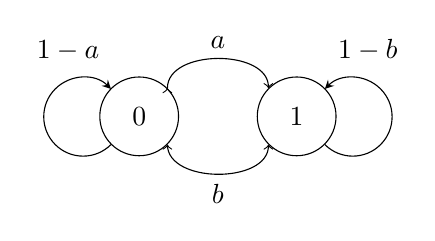
\begin{tikzpicture}
    [
      my circle/.style={minimum width=10mm, circle, draw},
      my label/.style={above=10pt, anchor=mid}
    ]
    \node[my circle] (1) at (-1,0) {$0$};
    \node[my circle] (2) at ( 1,0) {$1$};
    %\path [postaction={draw, {>[sep=5pt,reversed]}-{<[sep=5pt]}}, draw] (1) -- (2) node [very near start, my label] {$a$}  node [very near end, my label] {$\beta$} ;
		\path[->,draw] (1.south east)  edge[bend right=90] node [below] {$b$} (2.south west);
		\path[->,draw] (1.north east)  edge[bend left=90] node [above]  {$a$} (2.north west);
		\path [-stealth, draw] (2.south east) arc (-135:135:5mm) node [near end, my label] {$1-b$};
    \path [-stealth, draw] (1.south west) arc (-45:-315:5mm) node [near end, my label] {$1-a$};
  \end{tikzpicture}
	\caption{A two-state Markov chain}
	\label{fig:2sMC}
\end{figure}
For a two state \gls{mc} like the one in \ref{fig:2sMC}, we can write:
\begin{equation}\begin{split}
	f_{01}(n)&= P_{01} \cdot \delta(n-1) + P_{00} \cdot f_{01}(n-1) = a \cdot \delta(n-1) + (1-a)\cdot f_{01}(n-1)\\
	f_{01}(1)&=a \quad f_{01}(2)=a \cdot(1-a) \quad \dots \quad f_{01}(n) = a\cdot(1-a)^{n-1} n \ge 1 \\
	f_{11}(n) &= P_{11}\cdot \delta(n-1) + P_{10} \cdot f_{01}(n-1) =
	\begin{cases}
		1-b & n=1 \\ (1-a)^{n-2}\cdot a \cdot b & n>1
	\end{cases}
\end{split}\end{equation}

For a general \gls{mc}, we have
\begin{equation}\begin{split}
	P^{(n)} &= P^n \\
	P_{i,j}^{(n)} &= \sum\limits_{m=1}^n f_{i,j}(m) \cdot P_{j,j}^{(n-m)} \quad n \ge 1 \\
	f_{i,j}(n)&=
	\begin{cases}
		P_{i,j}^{(n)} -\sum\limits_{m=1}^{n-1} f_{i,j}(m) \cdot P_{j,j}^{(n-m)} & n \ge 2 \\
		P_{i,j}^{(n)} = P_{i,j} & n =1 \\
		0 & n=0
	\end{cases} \\
	\theta_{i,j}(n)&=
	\begin{cases}
		1 & \text{w.p. } P_{i,j} \\
		1+\theta_{k,j} &  \text{w.p. } P_{i,j} \text{ with } k \neq j
	\end{cases} \\
\end{split}\end{equation}

Let's now focus on the expectation of $\theta_{i,j}$. We can write:
\begin{equation}\begin{split}
	\exp[\theta_{i,j}] &= P_{i,j} + \sum\limits_{k \neq j} (1+\exp[\theta_{k,j}])\cdot P_{i,k}\\
	&\stackrel{(1)}{=} 1+ \sum\limits_{k \neq j} \exp[\theta_{k,j}] \cdot P_{i,k} \forall i \neq j\\
\end{split}\end{equation}
with \textit{(1)} $P_{i,j} + \sum\limits_{k\neq j}P_{i,k} =\sum\limits_{\forall k}P_{i,k} = 1 $
\\
We then get $N$ equations in $N$ unknowns, so the system can be solved.
\\
Now, with the example of the two state MC, we will show that the average return
time is the inverse of the in-state remaining probability.
\begin{equation}\begin{split}
	\exp[\theta_{0,1}] &= 1 + P_{00} \cdot \exp[\theta_{0,1}] \quad \exp[\theta_{0,1}] = \frac{1}{1-P_{00}} = \frac{1}{a}\\
	\exp[\theta_{1,0}] &= 1 + P_{11} \cdot \exp[\theta_{1,0}] \quad \exp[\theta_{1,0}] = \frac{1}{1-P_{11}} = \frac{1}{b}\\
	\exp[\theta_{0,0}] &= 1 + P_{01} \cdot \exp[\theta_{1,0}] =1+\frac{a}{b} = \frac{1}{1-P_{00}} = \left(\frac{b}{a+b}\right)^{-1}\\
	\exp[\theta_{1,1}] &= 1 + P_{10} \cdot \exp[\theta_{0,1}] =1+\frac{b}{a} = \frac{1}{1-P_{00}} = \left(\frac{a}{a+b}\right)^{-1}\\
	\lim_{n \to +\infty} P^n &=
	\begin{pmatrix}
		\frac{b}{a+b} & \frac{a}{a+b} \\
		\frac{b}{a+b} & \frac{a}{a+b}
	\end{pmatrix}
\end{split}\end{equation}

Analyzing the second order momentum, we have
\begin{equation}\begin{split}
	\exp[\theta_{i,j}^2] &= P_{i,j} + \sum\limits_{k \neq j} \exp[(1+\theta_{k,j})]\cdot P_{i,k}\\
	&= 1 + 2 \underbrace{\cdot \sum\limits_{k \neq j} \exp[\theta_{k,j}]\cdot P_{i,k}}_{\exp[\theta_{i,j}-1]} + \sum\limits_{k \neq j} \exp[\theta_{k,j}^2] \cdot P_{i,k}\\
	&= 2 \cdot \exp[\theta_{i,j}]-1 +  \sum\limits_{k \neq j} \exp[\theta_{k,j}^2] \cdot P_{i,k} \forall i \neq j \\
\end{split}\end{equation}

Which means that for the two-state MC, we have
\begin{equation} \begin{split}
	\exp[\theta_{01}^2] &= \frac{2 \cdot \exp[\theta_{01}]}{1-P_{00}} = \frac{\frac{2}{a}-1}{a} = \frac{2}{a^2} - \frac{1}{a}\\
	var[\theta_{01}] &= \frac{1-a}{a^2} \quad \text{same variance as a geometric r.v.} \\
	var[\theta_{10}] &= \frac{1-b}{b^2}\\
	\exp[\theta_{00}^2] &= 2 \cdot \exp[\theta_{00}]  -1 - P_{01}\cdot \exp[\theta_{10}^2] = 1 + \frac{a}{b} + \frac{2a}{b^2} \\
	var[\theta_{00}] &= \frac{a \cdot(2-a-b)}{b^2}\\
	var[\theta_{11}] &= \frac{b\cdot(2-a-b)}{a^2}\\
\end{split}\end{equation}

\subsection{Techniques to set up P matrix}
In this part, we will show some tips to set the P matrix, so that the solving and the product
will be easier when analyzing absorption time. First of all, you should discriminate
transient state and the one that creates the absorbing states, like the following:
\begin{equation} \begin{split}
	P&=\raisebox{-1\baselineskip}{\begin{blockarray}{cc}
      \begin{block}{(cc)}
          Q  & R \\
          0  & I \\
      \end{block}
			\parbox[c]{1.7cm}{\small 0,1,\dots,r-1 \text{transient}} & \parbox[c]{1.7cm}{\small r,\dots,n \text{absorbing}}
    \end{blockarray}}
	P^2 &= P \cdot P = \begin{pmatrix}
	Q^2 & Q \cdot R + R \\
	0 & I
	\end{pmatrix}	\\
\end{split}\end{equation}
which means that for the general case we have:
\begin{equation} \begin{split}
	P^n &= \begin{pmatrix}
	Q^n & \sum\limits_{i=0}^{n-1}Q^i \cdot R \\
	0 & I
	\end{pmatrix}
\end{split}\end{equation}
Let's now define $W_{i,j}^{(n)}$ as follows
\begin{definition}
	\begin{equation}
		W_{i,j}^{(n)} = \exp[\sum\limits_{l=0}^n \Chi \{ X_l=j\}|X_0=i] = \sum\limits_{l=0}^n\exp[\Chi \{ X_l=j\}|X_0=i]\sum\limits_{l=0}^n P_{i,j}^{(l)}
	\end{equation}
\end{definition}
Now suppose that $i,j$ are transient and put $W_{i,j}^{(n)}$ as element of a matrix. The resulting matrix will be:
\begin{equation}\begin{split}
	W^{(n)} &= I + Q + \dots + Q^n = I + Q \cdot W^{(n-1)} \\
	W &= \lim_{n \to +\infty} W^{(n)} = \sum\limits_{l=0}^{+\infty} [I-Q]^{-1} \cdot \vec{1}
\end{split}\end{equation}
If we sum, for all j transient states $W_{i,j}$  we obtain:
\begin{equation}
	\sum\limits_{j=0}^{r-1}W_{i,j} = \exp[\sum\limits_{n=0}^{T-1}\sum\limits_{j=0}^{r-1}\Chi\{X_n=j\}|X_0=i] = \exp[T|X_0=i]=v_i
\end{equation}
Let's now find the probability to go from a transient state ($i$) to an absorbing one($k$)
\begin{equation}
	U_{i,k}^{(n)} = \prob[T \le n , X_T = k | X_0=i] = \prob[X_n=k|X_0=i]=P_{i,k}^{(n)}
\end{equation}
This means that:
\begin{enumerate}
	\item $U^{(n)} = W^{(n-1)}\cdot R$
	\item $U=\lim_{n\to +\infty} U^{(n)} = W \cdot R = [I-Q]^{-1}\cdot R$
	\item $\tilde{P}=\begin{matrix} Q & r \\ \vec{0}&1 \end{matrix}$
\end{enumerate}
In conclusion, we found that the average first passage time is equal to the average
 absorption time, which is $[I-Q]^{-1}\cdot \vec{1}$
\section{Long Run Behaviour}
\subsection{Steady-state probabilities}

	\begin{definition}[Regular \gls{mc}]
		A regular \gls{mc} is a \gls{mc} with the following property:

		\begin{equation} \lim_{n \to \infty} P_{ij}^{(n)} = \lim_{ n \to \infty} Prob[ X_n=j | X_0 =i] = \pi_j > 0 \quad \forall i, j \end{equation}

	\end{definition}

	This tell us that:
	\begin{enumerate}
		\item Limit \textbf{exists} (not obvious)
		\item Limit is indipendent of the initial state
		\item Limit is \textbf{strictly} positive
	\end{enumerate}

	\begin{theorem}
		For a regular \gls{mc} with states 0, 1, ..., N the limit distribution $\bm\pi = (\pi_0,\pi_1,\cdots,\pi_N)$ is the unique solution of the following system of equations:\\

		$\begin{cases}
			\pi_j = \sum\limits_{k=0}^N \pi_k P_{k j} & \text{for } j = 0,1, \cdots, N \\
			\sum\limits_{k=0}^N \pi_k = 1\\
			\\ \pi_k \ge 0 & \forall k
		\end{cases}$
	\end{theorem}

	\begin{proof} of \textbf{existence}:
		\begin{equation}
  			P_{i j}^{(n)} = \sum\limits_{k=0}^N P_{ik}^{(n-1)} P_{k j}
			\qquad with ~\sum\limits_{k=0}^N P_{ik}^{(n)} = 1 ~\forall n
		\end{equation}
		it's the developing of $\bm P^n = \bm P^{n-1} \bm P$

		Now let's study what happens as $ n \to \infty $:
		\begin{equation}
			\begin{split}
				&\pi_j = \lim_{n \to \infty} P_{ij}^{(n)} = \lim_{n \to \infty} \sum\limits_{k=0}^N P_{ik}^{(n-1)} P_{k j
				} =\\
				&= \sum\limits_{k=0}^N \lim_{n \to \infty} P_{ik}^{(n-1)} P_{k j
				} = \sum\limits_{k=0}^N \pi_k P_{kj}
			\end{split}
		\end{equation}
		Here the limit and the sum can be switched since the sum is finite.
		This shows that the system have a solution.
	\end{proof}

	\begin{proof} of \textbf{uniqueness}:
		Let $X_j$ be a solution, so, by construction, $X_j = \sum\limits_{k=0}^N X_k P_{kj} ~$.

		For a given state $l$, it holds that
		\begin{equation}
				X_l = \sum\limits_{j=0}^N X_j P_{jl} =  \sum\limits_{j=0}^N \left( \sum\limits_{k=0}^N X_k P_{kj} \right) P_{jl} =  \sum\limits_{k=0}^N X_k \sum\limits_{j=0}^N P_{kj} P_{jl} = \sum\limits_{k=0}^N X_k P_{kl}^{(2)}
		\end{equation}

		If we apply this trick again $n$ times we can prove by induction that:
		$X_j$ also satisfy $ X_j = \sum\limits_{k=0}^N X_k P_{kj}^{(n)} $ \quad  $\forall n $

		Now, as $n \to \infty$, we have that
		\begin{equation}
			X_j = \sum\limits_{k=0}^N X_k \pi_j = \pi_j (\sum\limits_{k=0}^N X_k) = \pi_j  \implies
			\text{The solution is unique}
		\end{equation}
	\end{proof}

\subsection{Classes of states}
	\begin{definition}[Accessible State]
		State $j$ is {\bfseries accessible} from state $i$ if $\exists n \geq 0$ such that $P_{ij}^{(n)} > 0$. It can be written ($i \rightarrow j$).
		State it's \textbf{not} accessible if $\forall n \ge 0 \quad P_{ij}^{(n)}=0$
	\end{definition}

	\begin{definition}[Communicant States]
		States $i$ and $j$ are said to {\bfseries communicate}, written $ i \leftrightarrow j$, if
		$$\begin{cases}
			i \rightarrow j \\
			j \rightarrow i
		\end{cases}$$
	\end{definition}

	{\bfseries Proprieties}
	\begin{enumerate}
		\item \textbf{Reflexivity}: \quad $i \leftrightarrow i \quad\text{ given } P_{ii}^{(0)}=1$
		\item \textbf{Symmetry}: \quad if $i \leftrightarrow j$ then $j \leftrightarrow i$
		\item \textbf{Transitivity}: \quad if $i \leftrightarrow j$ and $j \leftrightarrow k \Rightarrow i \leftrightarrow k$
	\end{enumerate}
	This implies that communication between states is an equivalence relation.

	\begin{definition}[Periodicity]
		The period of state i, written $d(i)$, is the GCD (greatest common denominator) of set $S_i = \{ s>0 : P_{ii}^{(s)} >0 \}$.\\
		If $d(i)=1$, the state is said to be \textbf{aperiodic}.
	\end{definition}

	\begin{theorem}[Periodicity] Periodicity is a characteristic of groups (called \emph{classes}) of communicating states.
		$$\text{if } i \leftrightarrow j \text{, then } d(i) = d(j)$$
	\end{theorem}

	\begin{proof}
		Given $S_i = \{ s>0 : P_{ii}^{(s)} >0 \}$, and let $n, m > 0 : P_{ij}^{(m)} > 0, P_{ji}^{(n)} > 0$, we have that $$\forall s \in S_i : P_{ii}^{(s)} > 0$$

		Now, for total probability theorem, it holds that
		$$ P_{jj}^{(n+s+m)} = \sum\limits_{h, k} P_{jh}^{(n)} P_{hk}^{(s)} P_{kj}^{(m)} \geq P_{ji}^{(n)} P_{ii}^{(s)} P_{ij}^{(m)} >0 $$
		$$ P_{jj}^{(n+s+m)} >0 \implies n+s+m \in S_j$$

		$$P_{jj}^{(n+2s+m)} \geq P_{ji}^{(n)} P_{ii}^{(s)} P_{ii}^{(s)} P_{ij}^{(m)} >0 \Rightarrow n+2s+m \in S_j$$

		Now let's call $d(j) =$ g.c.d. of $S_j$.

		Since both $n+s+m$ and $n+2s+m$ are integer multiples of $d(j)$, so it is their difference $s$.

		We have proved that $\forall s \in S_i$ is integer multiple of $d(j)$: this implies that $d(j)$ is a common divisor of $S_i$, and moreover it divides the g.c.d. of $S$, $d(i)$. In conclusion, $d(i)$ is an integer multiple of $d(j)$.

		Doing this proof again switching role of $i$ and $j$ we prove that $d(j)$ is an integer multiple of $d(i)$, and so $d(i) = d(j)$.
	\end{proof}
	---

	\begin{definition}[Return Time]
		The random variable $R_i$ is defined as the time it takes to return to $i$ starting from $i$ itself.
	\end{definition}

	So the probability of ever going back to state $i$ can be written as
	$$ f_{ii} = \sum\limits_{n=1}^{+\infty} f_{ii}(n)  = \sum\limits_{n=1}^{+\infty} \prob[R_i=n | X_0=i] $$
	where $f_{ii}(n)$ is the probability of returning to state $i$ in $n$ steps.

	\begin{definition}[Recurrent state]
		A state is recurrent if $f_{ii} = 1$
	\end{definition}
	In other words we say that a state $i$ is recurrent if and only if, after the process starts from state $i$, the probability of its returning to state i after some finite length of time is one.

	\begin{definition}[Transient state]
		A state is transient if  $f_{ii} < 1$
	\end{definition}

	In other words a state $i$ is said to be transient if there exists a non-zero probability of never coming back to it.\footnote{like Angela. Please come back Angela, I love you.}

	\begin{definition}
		$M$ is the number of returns to state $i$, starting from $i$
		$$\exp[M | X_0 = i] = \sum\limits_{k=1}^{+\infty} \prob[M\geq k | X_0 = i] = \sum\limits_{k=1}^{+\infty} f_{ii}^k = \begin{cases}
		\frac{f_{ii}}{1-f_{ii}}, & \text{if transient} \\
		\infty, & \text{if recurrent}
		\end{cases}$$
	\end{definition}

	\begin{definition}[Proper r.v]
		given X a finite value r.v. it is called proper if $$\lim_{a\to \infty} \prob[X\geq a] = 0$$
	\end{definition}

	\begin{definition}[Improper r.v]
		given X a r.v. it is called improper if  $$\lim_{a\to \infty} \prob[X\geq a] = p_\infty \ne 0$$
	\end{definition}

	\begin{theorem}
		$$i  \text{ is recurrent} \iff \sum\limits_{n=1}^{+\infty} P_{ii}^{(n)} = \infty$$
	\end{theorem}
	---

	\begin{proof}
		Let the number of time state i has been visited be $$M = \sum\limits_{n=1}^{+\infty} \mathds{1}\{X_n =i\} $$
		The following swap from expected value and infinite sum is allowed by Fubini's Theorem
		$$
			\exp[M | X_0 = i] = \exp\left[\sum\limits_{n=1}^{+\infty} \mathds{1}\{X_n = i\} | X_0 = i\right]
			= \sum\limits_{n=1}^{+\infty} \exp\left[\mathds{1}\{ X_n = i\} | X_0 = i\right] = \sum\limits_{n=1}^{+\infty} P_{ii}^{(n)}
		$$
		So we have shown that $\exp[M | X_0=i] = \sum\limits_{n=1}^{+\infty} P_{ii}^{(n)}$.\\
		Now, remembering that $$ \exp[M | X_0 = i] = \begin{cases}
		\frac{f_{ii}}{1-f_{ii}}, & \text{if transient} \\
		\infty, & \text{if recurrent}
		\end{cases}$$
		the proof is concluded.
	\end{proof}

	\begin{theorem}
		(not to confuse with theorem on periodicity)
		$$\text{if } i\leftrightarrow j \text{and i is recurrent} \Rightarrow \text{ j is also recurrent}$$
	\end{theorem}
	---
	\begin{proof}
		$$\text{Since } i\leftrightarrow j : \exists m,n \text{ such that } P_{ij}^{(n)} \text{ and } P_{ji}^{(m)} > 0$$
		$$\text{let } r>0 : P_{jj}^{(m+r+n)} = \sum\limits_{r, k} P_{jh}^{(m)} P_{hk}^{(r)} P_{kj}^{(n)} \geq P_{ji}^{(m)}  P_{ii}^{(r)}  P_{ij}^{(n)}$$
		$$\sum\limits_{l=1}^{+\infty} P_{jj}^{(l)} \geq \sum\limits_{r=1}^{+\infty} P_{jj}^{(m+r+n)} \geq \sum\limits_{r=1}^{+\infty} P_{ji}^{(m)}  P_{ii}^{(r)}  P_{ij}^{(n)} = P_{ji}^{(m)} P_{ij}^{(n)} \sum\limits_{r=1}^{+\infty} P_{ii}^{(r)}$$
		but since \begin{itemize}
		\item$i$ is recurrent $\Rightarrow \sum\limits_{n=1}^{+\infty} P_{ii}^{(n)} = \infty$
		\item $P_{ij}^{(n)} \text{ and } P_{ji}^{(m)} > 0$
		\end{itemize}
		$$\sum\limits_{l=1}^{+\infty} P_{jj}^{(l)} = \infty \Rightarrow j \text{ is recurrent}$$
  \end{proof}

	\begin{theorem}[Basic limit theorem on MC] \label{th:basic_limit_MC}
		Consider an irreducible aperiodic recurrent MC (an aperiodic recurrent class), we have
		$$ \lim_{n\to \infty} P_{ii}^{(n)} = \frac{1}{m_i} = \pi_i = \lim_{n\to\infty} P_{ji}^{(n)} \qquad \forall j$$
	\end{theorem}
	---

	The following table summarize some properties for the types of state that can be found in a \gls{mc}:

	{\renewcommand{\arraystretch}{1.2}
	\begin{center}
		\begin{tabular}{|c||c|c|c|}
			\hline
			State $i$ & Transient & Null recurrent & Positive recurrent \\ \hline
			$f_{ii} = \sum\limits_{n=1}^{+\infty} f_{ii}^{(n)}$ & $<1$ & 1 & 1 \\ \hline
			$\lim\limits_{k \to \infty } \prob[M \geq k | X_0=i]$ & 0 & 1 & 1 \\ \hline
			$\exp[n|X_0=i]$ & $\frac{f_{ii}}{1-f_{ii}}$ & $\infty$ & $\infty$ \\ \hline
			$m_i = \sum\limits_n f_{ii}^{(n)}$ & $\infty$ & $\infty$ & $<\infty$ \\ \hline
			$\pi_i = \frac{1}{m_i}$ & 0 & 0 & $>0$ \\ \hline %positive. \pi is less than 1 and greater than 0
		\end{tabular}
	\end{center}}

	\begin{theorem}[1.3 (K.T. pp 85-86)]
		For an aperiodic positive recurrent class (irreducible MC), $\pi_j$ is the unique solution of the following system.
		\begin{equation*}\begin{cases}
			\pi_j = \sum\limits_{i=0}^{+\infty} \pi_i P_{ij} \\
			\sum\limits_{i=0}^{+\infty} \pi_i = 1 \\
			\pi_i \geq 0 \quad \forall i
		\end{cases}\end{equation*}
	\end{theorem}

	\begin{proof} The funny thing is that this proof is easier than the book.
		It is splitted in several parts, as can be noticed.

		\proofpart
			We first want to show that the $\pi_j$ satisfy the system (\textbf{\textit{Existence of the solution}})
			\begin{equation*}
				\begin{split}
					\forall m,n \qquad 1&=\sum\limits_{j=0}^{+\infty} P_{ij}^{(n)} > \sum\limits_{j=0}^m P_{ij}^{(n)}\\
	 			 \lim_{n\to\infty} \sum\limits_{j=0}^m P_{ij}^{(n)} &= \sum\limits_{j=0}^m \pi_j \leq 1 \quad \forall n \\
				 &\implies \sum\limits_{j=0}^{+\infty} \pi_j \leq 1\\
				\end{split}
			\end{equation*}

		\proofpart
			\begin{equation*}
				\begin{split}
					P_{ij}^{(n+m)} &\geq \sum\limits_{k=0}^m P_{ik}^{(m)} P_{kj}^{(n)} \quad \forall n, m, M\\
					\text{as } m \to \infty :\quad \pi_j &\geq \sum\limits_{k=0}^m \pi_k P_{kj}^{(n)}\\
					&\implies  \pi_j \geq \sum\limits_{k=0}^m \pi_k P_{kj}^{(n)}
				\end{split}
			\end{equation*}

		\proofpart
			\begin{equation*}
				\begin{split}
					\sum\limits_{k=0}^{+\infty} \sum\limits_{j=0}^{+\infty} \pi_k P_{kj}^{(n)} &\geq
					\sum\limits_{k=0}^m \sum\limits_{j=0}^{+\infty} \pi_k P_{kj}^{(n)}  \\
					&=(\text{since } \sum\limits_{j=0}^{+\infty} P_{kj}^{(n)} = 1 )\\
					&=\sum\limits_{k=0}^m \pi_k \quad \forall m\\
					\text{suppose } \exists j > 1 : \pi_j &> \sum\limits_{k=0}^{+\infty} \pi_k P_{kj}^{(n)} \\
					\text{then we have that } \sum\limits_{j=0}^{+\infty} \pi_k &> \sum\limits_{j=0}^{+\infty} \sum\limits_{k=0}^{+\infty} \pi_k P_{kj}^{(n)} > \sum\limits_{k=0}^{+\infty} \pi_k \quad \text{ABSURD.} \\
					&\implies \pi_j = \sum\limits_{k=0}^{+\infty} \pi_k P_{kj}^{(n)}
				\end{split}
			\end{equation*}

		\proofpart
			\begin{equation*}
				\begin{split}
			 		\pi_j = \sum\limits_{k=0}^{+\infty} \pi_k P_{kj}^{(n)}, \qquad |P_{kj}^{(n)}| &\leq 1 \quad \forall n,i,k \\
					\text{using an appropriate theorem for sliding the}&\text{ limit inside the infinite sum we have:}\\
					\pi_j = \sum\limits_{k=0}^{+\infty}  \pi_k \lim_{n\to\infty} P_{kj}^{(n)} &= (\sum\limits_{k=0}^{+\infty} \pi_k) \pi_j\\
					\text{and now since $\pi_j>0$}
					&\implies \sum\limits_{k=0}^{+\infty} \pi_k = 1
				\end{split}
			\end{equation*}
			\textbf{\textit{This concludes the existence proof.}}

		\proofpart
			Let's now prove the \textbf{\textit{Uniqueness}} \\
			Suppose $X_j$ is a solution
			\begin{equation}
				\begin{split}
					X_j =
					 \sum\limits_{i=0}^{+\infty} X_i P_{ij} &=
					 \sum\limits_{i=0}^{+\infty} ( \sum\limits_{k=0}^{+\infty} X_k P_{ki} ) P_{ij} \geq
					 \sum\limits_{k=0}^m X_k \\
					 \sum\limits_{i=0}^{+\infty} P_{ki} P_{ij} &= \sum\limits_{k=0}^m X_k P_{kj}^{(2)}
					 \quad \forall m
					 \Rightarrow X_j \geq \sum\limits_{k=0}^{+\infty} X_k P_{kj}^{(n)}\qquad \forall n
				\end{split}
			\end{equation}

			This is the same result of $3^{rd}$ step, so as in $3^{rd}$ step, we can prove by contradiction that this inequality is in fact an equality.

			$$ \implies X_j = \sum\limits_{k=0}^{+\infty} X_k P_{kj}^{(n)} \quad \forall n $$
			as $n \to \infty$ we have:

			\begin{equation}
				X_j = (\sum\limits_{k=0}^{+\infty} X_k ) \pi_j \Rightarrow X_j = \pi_j
			\end{equation}

			So it's unique.
	\end{proof}

	\begin{lemma}
	  If $0 < p_i < 1 ~,~ i=0,1,2.\cdots $, then:
		\begin{equation}\label{limprodpi}
			\lim_{m \to \infty} \prod_{i=0}^{m}(1-p_i) = 0
		\end{equation}
		if and only if
		\begin{equation}\label{pitoinfty}
			\sum\limits_{i=0}^{+\infty} p_i = \infty
		\end{equation}
	\end{lemma}

	\begin{proof}
		\begin{enumerate}
			\item Assume \eqref{pitoinfty} is true. \\
				Since the series expansion for $e^{-p_i}$ is an alternating series with terms decreasing in absolute value, we can write:
				\begin{equation}
					1-p_i < 1-p_i + \frac{p_i^2}{2!} - \frac{p_i^3}{3!} + \cdots = ~e^{-p_i} \quad with ~i\ge 0
				\end{equation}
				applying the product to both members we obtain
				\begin{equation}
					\prod_{i=0}^{k-1} (1-p_i) < e^{-\sum\limits_{i=0}^{k-1}p_i}
				\end{equation}
				But by assumption $\sum\limits_{i=0}^{+\infty} p_i = \infty$ hence,
				$$ \lim_{m \to \infty} \prod_{i=0}^{m}(1-p_i) = 0 $$

			\item Let's prove the following inequality:
			$$ \prod_{i=j}^m(1-p_i) > 1-\sum\limits_{i=j}^m p_i \quad \forall m \ge j+1$$
			We can prove it recursively:
			$$(1-p_j)(1-p_{j+1}) = 1-p_j - p_{j+1} + p_j p_{j+1} > 1-p_j - p_{j+1}$$
			Iterating we obtain:
			\begin{eqnarray*}
				\prod_{i=j}^{m+1}(1-p_i) = (1-p_{m+1})\prod_{i=j}^m(1-p_i) > (1-p_{m+1})(1-\sum\limits_{i=j}^m p_i) = \\
				1- \sum\limits_{i=j}^{m+1} p_i + p_{m+1}\sum\limits_{i=j}^m p_i
			\end{eqnarray*}

			Assume now that $\sum\limits_{i=1}^{+\infty} p_i < \infty$, then there must exist an index $j>1$ s.t. $\sum\limits_{i=j}^{+\infty} p_i < 1$.

			Then we have:
			$$ \lim_{m \to \infty} \prod_{i=j}^m (1-p_i) \ge \lim_{m \to \infty} (1-\sum\limits_{i=j}^m p_i) > 0 $$
		\end{enumerate}
	\end{proof}

	\begin{definition}[lesson 22/03/17] \label{def:falling_probability}
		Given a recurrent class $C$ and a transient state $i \notin C$, the probability of entering in that class through state $k \in C$ at step $n$ can be written as
		$$ \pi_{ik}^{(n)}(C) = \prob[X_n = k \in C, x_l \notin C ~ \forall l=1, ..., n-1 | X_0 = i] $$

		Thus, the probability that the chain, starting from $i$, reaches class $C$ at step $n$ is
		$$ \pi_{i}^{(n)}(C) = \sum_{k \in C} \pi_{ik}^{(n)}(C) $$

		and the general probability of reaching $C$ starting from $i$ is
		$$ \pi_i(C) = \sum_{n \in \N} \pi_i^{(n)}(C) $$
	\end{definition}

	\begin{theorem}[3.1, KT p. 91] \label{th:3.1}
		Given state $j \in C$, an aperiodic and recurrent class, and a transient state $i \notin C$, it holds that

		$$ \lim_{n \to \infty } P_{ij}^{(n)} = \pi_i(C) \cdot \lim_{n \to \infty } P_{jj}^{(n)} = \pi_i(C) \cdot \pi_j $$
	\end{theorem}
	---
	\begin{proof}
		The limit of theorem thesis can be expanded this way
		\begin{equation}\begin{split} \label{eq:theorem_3.1_thesis}
			& \forall \epsilon > 0, \exists \text{ class } C' \in C, N \in \N \text{ such that } \\
			& \forall n \ge N,~ \left| P_{ij}^{(n)} - \pi_i(C) \pi_j \right| \stackrel{(1)}{=} \\
			= & \left| P_{ij}^{(n)} - \left( \sum_{v = 1}^{N} \sum_{k \in C'} \pi_{ik}^{(v)}(C) \right) \pi_j +
				\left( \sum_{v = 1}^{N} \sum_{k \in C'} \pi_{ik}^{(v)}(C)\right)\pi_j - \pi_i(C)\pi_j \right| \stackrel{(2)}{\le} \\
			\le & \left| P_{ij}^{(n)} - \left( \sum_{v = 1}^{N} \sum_{k \in C'} \pi_{ik}^{(v)}(C) \right) \pi_j \right| +
				\left| \left( \sum_{v = 1}^{N} \sum_{k \in C'} \pi_{ik}^{(v)}(C)\right) - \pi_i(C) \right| \pi_j
		\end{split}\end{equation}
		where
		\begin{itemize}
			\item [(1)] term between parenthesis is added and subtracted
			\item [(2)] absolute value of a sum is less or equal than the sum of the absolute values
		\end{itemize}

		If we can prove that the two terms are infinitesimal (i.e. $< \epsilon$) for given $N$ and $C'$, we are done.
		\smallbreak

		First we can prove that, given class $C$ is recurrent, transition probability in $n$ steps from $i$ to $j$ can be formulated as follows.
		\begin{equation} \label{eq:n_step_in_class}
			P_{ij}^{(n)} = \sum_{v = 1}^{n} \sum_{k \in C} \pi_{ik}^{(v)}(C) ~ P_{kj}^{(n-v)}
		\end{equation}
		where path from $i$ to $j$ is splitted in two parts, before and after entering $C$.

		This formula can be written as a limit in $n$ and $C$, expliciting the inner infinite sum over class elements.

		% FORMAT setting
		\setlength{\mathindent}{-1.5cm} % sporco trucco ingegneristico

		\begin{equation}\begin{split} \label{eq:theorem_3.1_first term}
			& \forall \epsilon > 0, \exists N \in \N \text{ and a finite class } C' \subseteq C \text{ such that } \\
			& \forall n \ge N, \left| P_{ij}^{(n)} - \pi_j \left( \sum_{v = 1}^{n} \sum_{k \in C'} \pi_{ik}^{(v)} \right) \right| \stackrel{(1)}{=}
			\\
			= & \left|
				\left(
					\sum_{v = 1}^{n} \sum_{k \in C'} \pi_{ik}^{(v)}(C) ~ P_{kj}^{(n-v)} + \sum_{v = 1}^{n} \sum_{\substack{k \in C \\ k \notin C'}} \pi_{ik}^{(v)}(C) ~ P_{kj}^{(n-v)} \right)
				- \pi_j \left( \sum_{v = 1}^{n} \sum_{k \in C'} \pi_{ik}^{(v)}(C) \right)
				\right| \stackrel{(2)}{=}
			\\
			= & \left| \sum_{v = 1}^{n} \sum_{k \in C'} \pi_{ik}^{(v)}(C) (P_{kj}^{(n-v)} - \pi_j)
				+ \sum_{v = 1}^{n} \sum_{\substack{k \in C \\ k \notin C'}} \pi_{ik}^{(v)}(C) P_{kj}^{(n-v)} \right| \stackrel{(3)}{=}
			\\
			= & \left| \sum_{v = 1}^{N} \sum_{k \in C'} \pi_{ik}^{(v)}(C) (P_{kj}^{(n-v)} - \pi_j) +
				\sum_{v = N+1}^{n} \sum_{k \in C'} \pi_{ik}^{(v)}(C) (P_{kj}^{(n-v)} - \pi_j) +
				\sum_{v = 1}^{n} \sum_{\substack{k \in C \\ k \notin C'}} \pi_{ik}^{(v)}(C) P_{kj}^{(n-v)} \right| \stackrel{(4)}{\le}
			\\
			\le & \left| \sum_{v = 1}^{N} \sum_{k \in C'} \pi_{ik}^{(v)}(C) (P_{kj}^{(n-v)} - \pi_j) \right| +
				\left| \sum_{v = N+1}^{n} \sum_{k \in C'} \pi_{ik}^{(v)}(C) (P_{kj}^{(n-v)} - \pi_j) \right| +
				\left| \sum_{v = 1}^{n} \sum_{\substack{k \in C \\ k \notin C'}} \pi_{ik}^{(v)}(C) P_{kj}^{(n-v)} \right| \stackrel{(5)}{\le}
			\\
			\le & \left| \sum_{v = 1}^{N} \sum_{k \in C'} \pi_{ik}^{(v)}(C) (P_{kj}^{(n-v)} - \pi_j) \right| +
				2 \left( \sum_{v = N+1}^{n} \sum_{k \in C'} \pi_{ik}^{(v)}(C) \right) +
				\left( \sum_{v = 1}^{n} \sum_{\substack{k \in C \\ k \notin C'}} \pi_{ik}^{(v)}(C) \right) \stackrel{(6)}{\le}
			\\
			\le & \left| \sum_{v = 1}^{N} \sum_{k \in C'} \pi_{ik}^{(v)} (P_{kj}^{(n-v)} - \pi_j) \right| + 3 \epsilon \stackrel{(7)}{<} 4 \epsilon
		\end{split}\end{equation}

		\setlength{\mathindent}{0cm} % reset of "sporco trucco ingegneristico"

		since $\pi_j = \lim_{n \to +\infty} P_{kj}^{(n-v)}$ by definition, what we have here is a finite sum (over $N$ and $C'$) of infinitesimal quantities
		where
		\begin{itemize}
			\item [(1)] using equation \eqref{eq:n_step_in_class}, sum is splitted in $k \in C$ into two sums in $k \in C'$ and $k \in C ~ \wedge ~ k \notin C' $
			\item [(2)] terms have been rearranged: first and last one have been merged
			\item [(3)] the first sum over all $n \in \N$ is splitted using $N$
			\item [(4)] the module of a sum is less or equal than the sum of the modules
			\item [(5)] given it always holds that $P_{kj}^{(n-v)} \le 1$ and $|P_{kj}^{(n-v)} - \pi_j| \le 2$
			\item [(6)] choosing $C'$ and $N$ large enough, we can make the two terms between parenthesis small as we want: they are infinitesimal
			\item [(7)] since $\pi_j = \lim_{n \to +\infty} P_{kj}^{(n-v)}$ by definition, what we have here is a finite sum (over $N$ and $C'$) of infinitesimal quantities
		\end{itemize}
		This way we have verified that first term of \eqref{eq:theorem_3.1_thesis} is in fact infinitesimal.

		\bigbreak
		Now we explore the second term.
		Given definitions \ref{def:falling_probability}, it holds that
		$$ \pi_i(C) = \sum_{v = 1}^{+\infty} \sum_{k \in C} \pi_{ik}^{(v)}(C) $$

		\smallbreak
		Since the right term converges to a finite value, namely $\pi_i$, the limit implicit in the infinite sum can be expanded this way.
		\begin{equation}\begin{split} \label{eq:pi_limit_definition}
			& \forall \epsilon > 0, \exists N \in \N \text{ and a finite class } C' \subseteq C \text{ such that } \\
			& \forall n \ge N,~ \left| \pi_i(C) - \sum_{v = 1}^{n} \sum_{k \in C'} \pi_{ik}^{(v)}(C) \right| < \epsilon
		\end{split}\end{equation}

		\bigbreak
		Recalling thesis (equation \eqref{eq:theorem_3.1_thesis}), both terms of the sum have been proven infinitesimal, so wanted limit is itself proven.
	\end{proof}

	Summarizing all we know about limiting distribution across multiple classes, we can build the following table.
	See theorem \ref{th:3.1} for last line.
	\begin{center}\begin{tabular}{c|c|c}
		Starting state $i$ & Arrival state $j$ & $\lim_{n \to +\infty} P_{ij}^{(n)}$ \\ \hline
		any & transient & 0 \\
		recurrent $\notin C' ,\: \in C$ & recurrent $\in C$ & 0 \\
		recurrent $\in C$ & recurrent $\in C$ & $\pi_j = 1 / m_j$ \\
		transient & recurrent $\in C$ & $\pi_i(C)\cdot\pi_j = \pi_i(C) / m_j$ \\
	\end{tabular}\end{center}

	\begin{theorem}[Property of finite \gls{mc}] \label{th:finite_MC_1}
		A finite \gls{mc} must have at least a positive recurrent state.

		$$ \forall \text{ finite \gls{mc}, } \exists i: \pi_i \neq 0 $$
	\end{theorem}
	---
	\begin{proof}
		Labeling \gls{mc} states from $1$ to $N$, we can always write that

		$$ \forall i, n ~ \sum_{j=0}^N P_{ij}^{(n)} = 1$$

		This holds for each value of $n$, so it must be true also in the limit.
		Suppose also that there are no positive reccurent states:
		$$ 1 = \lim_{n \to +\infty} \sum_{j=0}^N P_{ij}^{(n)} \stackrel{(*)}{=} \sum_{j=0}^N \lim_{n \to +\infty} P_{ij}^{(n)}
		= \sum_{j=0}^N \pi_j $$
		where passage marked with the (*) is possible only because sum is finite.

		Since the sum of the $\pi_j$ is not zero, one of them must be strictly positive.
		Corresponding state is then positive recurrent, proving our theorem.
	\end{proof}

	\begin{theorem}[Property of finite \gls{mc}]
		A finite \gls{mc} can't have null recurrent state.

		$$ \text{ In a finite \gls{mc}, } \nexists~ i: \pi_i = 0 $$
	\end{theorem}
	---
	\begin{proof}
		Supposing such a null recurrent exists, there must be a null recurrent class that contains it.
		Such class is finite, given the chain is finite too.

		But for theorem \ref{th:finite_MC_1} such class must have at least one positive recurrent state, which is absurd.
		So a null recurrent class cannot exist in a finite \gls{mc}.
	\end{proof}

	\begin{definition}
		Given a \gls{mc} with a state set $S = \{1, 2, ...\}$, quantity $Y_i(n)$ is defined as the probability of staying in $S$ along an $n$-steps path that starts from $i \in S$.

		$$ Y_i(n) = \prob[X_j \in S ~\forall j=1, 2, ..., n | X_0 = i \in S] $$
	\end{definition}

	\begin{theorem}
		$Y_i(n)$ is monothonically non-increasing on $n$.
		$$ Y_i(n) \le Y_i(n-1) $$
	\end{theorem}
	---
	\begin{proof} Base case $n=1$
		\begin{equation}\begin{split} \label{eq:Y_i-properties}
			& Y_i(1) = \prob[X_1 \in S | X_0 = i] = \sum_{j \in S} P_{ij} \\
			& Y_i(2) \stackrel{(*)}{=} \sum_{j \in S} P_{ij} Y_i(1) \le \sum_{j \in S} P_{ij} = Y_i(1)
		\end{split}\end{equation}
		where (*) holds by \emph{first step analysis}: $ Y_i(n) = \sum_{j \in S} P_{ij} Y_j(n-1) $.
	\end{proof}

	\begin{proof} Inductive step
		\begin{equation}\begin{split}
			& Y_i(n+1) \stackrel{(1)}{=} \sum_{j \in S} P_{ij} Y_i(n) \stackrel{(2)}{\le} \sum_{j \in S} P_{ij} Y_i(n-1) \stackrel{(3)}{=} Y_i(n)
		\end{split}\end{equation}
		where (1) and (3) hold by first step analysis and (2) for inductive hypothesis.
	\end{proof}

	\begin{lemma}
		Since $Y_i(n)$ is monothonically non-increasing and positive (it is a probability), we can always take the limit for $n \to +\infty$.

		$$ \exists \lim_{n \to +\infty} Y_i(n) \stackrel{.}{=} Y_i = \prob[\text{staying in } S | \text{starting from } i \in S] $$
		where $ S = \{ 1, 2, 3, ...\} $ as before.

		Using \emph{first step analysis} as in previous equation \eqref{eq:Y_i-properties} and taking the limit for $n \to +\infty $, we can build the following system.
		\begin{equation} \label{eq:Yj_system}
			\forall i \neq 0, Y_i = \sum_{j \in S} P_{ij} Y_j
		\end{equation}
	\end{lemma}

	\begin{lemma}
		Let $\{Z_i, i=1, 2, ...\}$ be a solution set for system \eqref{eq:Yj_system}. We focus in particular on non-divergent solutions, imposing that $ \forall i, |Z_i| \le 1 $.

		It holds that
		$$ \forall n, |Z_i| \le Y_i(n) ~ \Rightarrow ~|Z_i| \le \lim_{n \to +\infty} Y_i(n) = Y_i $$
	\end{lemma}
	---
	\begin{proof} Base case $n=1$
		$$ |Z_i| = \sum_{j \in S} P_{ij} |Z_j| \stackrel{(*)}{\le} \sum_{j \in S} P_{ij} = Y_i(1) $$
		where (*) holds because $|Z_i| < 1$.
	\end{proof}

	\begin{proof} Inductive step
		$$ |Z_i| = \sum_{j \in S} P_{ij} |Z_j| \stackrel{(*)}{\le} \sum_{j \in S} P_{ij} Y_j(n) = Y_i(n+1) $$
		where (*) is due to the inductive hypothesis.
	\end{proof}

	\begin{lemma}[4.13 (Ross 2, pg. 78-82)] \label{lemma:MC_irreducible_fi0}
		Given an irreducible \gls{mc} with a state set $S=\left\{0,1,2,\dots \right\}$ it is recurrent if and only if:

		$$ \forall i \neq 0, f_{i 0} = 1 $$
		where $f_{i 0}$ is the probability of reaching state $j$ starting from 0 at any time in the future.
	\end{lemma}
	---
	\begin{proof} \emph{if implication} $"\Leftarrow"$
		\begin{equation}\begin{split}
			f_{00} = P_{00} + \sum_{i \neq 0} P_{0i} f_{i 0} \stackrel{(*)}{=} \sum_{i} P_{0i} = 1
		\end{split}\end{equation}
		where (*) is due to hypothesis.

		This implies that, starting from any state $j$, the chain returns to zero eventually with probability 1.
	\end{proof}

	\begin{proof} \emph{only if implication} $"\Rightarrow"$
		Suppose chain is irreducible, but thesis is false, i.e.
		$$ \exists i \neq 0 : f_{i0} < 1 $$

		If \gls{mc} is irreducible (i.e. it is made only of a single class) it must be that
		$$ \forall i \neq 0, \exists m : P_{0i}^{(m)} > 0 $$

		Let $n$ be the minimum value among all possible $m$  that satisfies this condition for given state $i \neq 0$: such number is the shortest path from 0 to $i$ and, by its definition, does not cross state 0 in the middle.

		$$ \prob[\forall n, X_n \neq 0 | X_0 = 0] = 1 - f_{00} \stackrel{(*)}{\ge} P_{0i}^{(n)} (1 - f_{i0}) > 0 \Rightarrow \text{ state 0 is transient} $$

		where (*) inequality holds because leaving 0 forever (first term) is a more general case of going to state $i$ via the shortest path and then not crossing 0 ever again.

		This is absurd, because chain is supposed irreducible.
	\end{proof}

	\begin{theorem}[4.14]
		An irreducible \gls{mc} with states $S = 0, 1, 2, ...$ is transient if and only if

		$$ Z_i = \sum_{j=1}^{+\infty} P_{ij} Z_j \text{ for } i = 1, 2, ...$$

		has a non-zero bounded solution with $ |Z_i| \le 1$.
	\end{theorem}
	---
	\begin{proof}
		Let's consider a \gls{mc} and a state subset $S = \{1, 2, 3, ...\}$.

		$$ \prob[\text{leaving } S| X_0 = i \neq 0] \stackrel{(1)}{=}
			1 - Y_i \stackrel{(2)}{=} f_{i0} $$
		where (1) holds for $Y_i$ definition and (2) because, for $S$ formulation, leaving $S$ means reaching 0.

		We can now distinguish two cases, based on $Z_i$ solutions:
		\begin{itemize}
			% Z has only at most zero solutons
			\item $ \forall i, Z_i \le 0 \Leftrightarrow \forall i, Y_i = 0 \Leftrightarrow \forall i, f_{i0} = 1 \stackrel{(*)}{\Leftrightarrow} $ chain is recurrent

			% Z has a non zero bounded solution
			\item $ \exists i: Z_i > 0 \Leftrightarrow \exists i: Y_i > 0 \Leftrightarrow \exists i: f_{i0} < 1 \stackrel{(*)}{\Leftrightarrow} $ chain is transient
		\end{itemize}
		where (*) implications hold for theorem \ref{lemma:MC_irreducible_fi0}.
	\end{proof}

\subsection{M/G/1}
Let's now consider a queueing system where arrivals are markovian and there's only one server which acts with a generic proibability distribution. Let's then define the probability transition matrix as
\begin{equation}\label{eq:mg1P}
	P=\begin{pmatrix}
 \color{red}{a_o}& \color{blue}{a_1} & \color[rgb]{0,0.7,0}{a_2} & \dots &\dots & \\
 \color{red}{a_o}& \color{blue}{a_1} & \color[rgb]{0,0.7,0}{a_2}& \dots & \dots \\
 0  & \color{red}{a_o}& \color{blue}{a_1} & \color[rgb]{0,0.7,0}{a_2} & \dots \\
 0 & 0 & \color{red}{\ddots} & \color{blue}{\ddots} &\color[rgb]{0,0.7,0}{\ddots} \\
\vdots & \ddots &\ddots & \color{red}{\ddots} & \color{blue}{\ddots} &\color[rgb]{0,0.7,0}{\ddots} \\

\end{pmatrix}
\end{equation}

Let's now define the probability of moving to state $i$ in one step as
\begin{esp}\label{eq:MG1-intro}
	\Pi_i &= \sum\limits_{j=0}^{+\infty} \pi_j \cdot P_{ji} \quad \forall i \\
	\sum\limits_{i=0}^{+\infty} \pi_i &=1\\
	\sum\limits_{i=0}^{+\infty} a_i &=1
\end{esp}
Looking at P in \eqref{eq:mg1P} we can simplify the previous equation as
\begin{equation}
	\Pi_i = \Pi_o \cdot a_i +  \sum\limits_{j=0}^{i+1} \pi_j \cdot a_{i-j+1}\quad i \ge 0
\end{equation}
We can then see all $\Pi_i$ and $a_i$ as two Laplace transform, which means
\begin{esp}\label{eq:lsplaceMG1}
	\Pi(s) &= \sum\limits_{i=0}^{+\infty} \pi_i \cdot s^i \\
	A(s) &= \sum\limits_{i=0}^{+\infty} a_i \cdot s^i \\
\end{esp}
The generic term $a_{i+1}$ can be written as
\begin{equation*}
	\sum\limits_{i=0}^{+\infty} a_{i+1} \cdot s^i =\sum\limits_{i=1}^{+\infty} a_i \cdot s^{i-1} = \frac{A(s) - a_o}{s}
\end{equation*}
We can then write the convolution $()\pi * a) (i)$ as the product of the two Laplace transform calculated in equation \eqref{eq:lsplaceMG1}.

We can then write the Laplace transform of the $\Pi$ as
\begin{esp}
	\Pi(s) &= \pi_o \cdot A(s) + \frac{A(s) \cdot \Pi(s) - \pi_o a_o}{s} -\frac{A(s) \cdot \pi_o - \pi_o a_o}{s} \\
	s \cdot & \Pi(s) - A(s) \cdot \Pi(s) = \pi_o \cdot A(s) \cdot (s-1) \\
	\Pi(s) &= \pi_o \cdot \frac{A(s)\cdot(s-1)}{s - A(s)}
\end{esp}
Letting s go to 1 and reminding that A(1)=1 we can write
\begin{esp}\label{eq:s-to1}
	1=\lim_{s\to 1} \Pi(s) &= \pi_o \cdot \lim_{s\to 1} \frac{s-1}{s-A(s)} \\
	&=\pi_o \cdot \lim_{s\to 1} \left(1-\underbrace{\frac{A(s)-1}{s-1}}_{(1)}\right)^{-1} = \pi_o\cdot\left[1-A^{\prime}(1)\right]^{-1} = \frac{\pi_o}{1-A^\prime(1)}
\end{esp}
where $(1)$ can be seen as the definition of the derivative of A(s) calculated in s=1

We can then define
\begin{equation*}
	A^\prime(1) = \rho = \sum\limits_{n=0}^{+\infty} n \cdot a_n
\end{equation*}

rewriting \eqref{eq:s-to1}, we can say:
\begin{esp} \label{eq:pi0rho}
	1&= \frac{\pi_o}{1-\rho} \\ \Rightarrow & \pi_o = 1-\rho
\end{esp}
In case $\pi_o \notin [0;1]$ there's no solution to the system.\\
In conclusion we found that
\begin{equation}\begin{cases}
	0 \le \rho \le 1 & \Leftrightarrow \text{ positive recurrent} \\
	\rho>1 & \implies \text{ transient}
\end{cases}\end{equation}
Where the second equation is one-direction only because we cannot say that if I cannot find a solution by guess, then there's no solution.

\subsection{Random walks}
Let $0,1,2,\dots$ be the states that keep track of the random walk. Let's now define the probability to advance in state and going back to the previous state as follows:
\begin{esp}
	p_i &= P_{i i+1} \quad \text{probability to go $i\to i+1 $}\\
	q_i &= P_{i i-1} = 1-p_i \quad \text{probability to go $i\to i-1$ }\\
	\text{with } & p_o = 1 ~ q_o = 0
\end{esp}
Let's now define $Z_i$ the probability to reach state i from all the other states, which means
\begin{esp}
	Z_i &= \sum\limits_{i=1}^{+\infty} P_{i j} \cdot Z_j \\
	Z_1 = p_1 \cdot Z_2
\end{esp}
where with the last row we say that in one step the state can move upward or downward by only one state.

We can then write:
\begin{esp}
	\underbrace{p_i + q_i}_{=1} \cdot Z_i &= p_i \cdot Z_{i+1} + q_i \cdot Z_{i-1} \quad i>1 \\
	q_i \cdot\left(Z_i - Z_{i-1}\right) &=p_i \cdot\left( Z_{i+1} - Z_i \right)\\
	Z_{i+1} = Z_i + \frac{q_i}{p_i}\cdot \underbrace{\left(Z_i - Z_{i-1}\right)}_{(1)}
\end{esp}
where $(1)$ can be written as $\frac{q_{i-1}}{p_{i-1}} \left(Z_{i-1} - Z_{i-2}\right)$. \\

We can then write the recursive equation for $Z_i$ as follows
\begin{esp}
Z_{i+1} &= Z_i + Z_1 \cdot \prod\limits_{j=1}^i \frac{q_j}{p_j} \quad i \ge 1\\
Z_n+1 &= \sum\limits_{i=1}^n \left(Z_{i+1} - Z_i \right)	+Z_1 = Z_1 \cdot \sum\limits_{i=0}^{n} \prod\limits_{j=1}^i \frac{q_j}{p_j}
\end{esp}
Moreover we find that if $\sum\limits_{i=0}^{+\infty}p_i < \infty$ then there exists a non-zero bounded solution and therefore the \gls{mc} is transient.
The table \ref{tab:rw} summarize the result we just found
\begin{table}[]
\centering
\label{tab:rw}
\begin{tabular}{c|cc}
Cases \ series                                                & \multicolumn{1}{c|}{$\sum\limits_{i=0}^{+\infty} \prod\limits_{j=1}^i \frac{q_j}{p_j}$} & $\sum\limits_{i=0}^{+\infty} \prod\limits_{j=1}^i \frac{p_j}{q_{j+1}}$ \\ \hline
Transient                                                     & $< +\infty$                                                                             & $+\infty$                                                            \\
\begin{tabular}[c]{@{}c@{}}Positive \\ recurrent\end{tabular} & $+\infty$                                                                               & $< +\infty$                                                          \\
\begin{tabular}[c]{@{}c@{}}Null\\ recurrent\end{tabular}      & $+\infty$                                                                               & $+\infty$
\end{tabular}
\end{table}

We can then study the result obtained with what we found in M/G/1 system. We can see the $P_{i j}$ as the $a_i$, so we derive:
\begin{equation}
	Z_i = \sum\limits_{j=1}^{+\infty} P_{i j} \cdot Z_j = \sum\limits_{j=1}^{+\infty} a_{j} \cdot Z_j=\sum\limits_{j=0}^{+\infty} a_{j} \cdot Z_{i+j-1}
\end{equation}
If we consider $Z_i = 1-s$ we obtain that
\begin{equation}
	1-s = \sum\limits_{j=0}^{+\infty} a_{j} \cdot (1-s^j) \stackrel{(1)}{=}\sum\limits_{j=1}^{+\infty} a_{j} \cdot (1-s^j) = 1-A(s)
\end{equation}
where $(1)$ is possible as $s^0=1$, so the first term of the sum is null.

We then found out that $A(s)=s$. We can then calculate:
\begin{equation}
	1-s^i = \sum\limits_{j=0}^{+\infty} a_{j} \cdot (1-s^{i+j-1}) = 1-s^{i-1} \cdot A(s)
\end{equation}

but I don't know why. TODO!!

\begin{theorem}[4.2, KT p. 95 (sufficient condition for recurrence)]
	An irreducible \gls{mc} is recurrent if:

	\begin{equation}\noindent
		\exists \text{ a sequence } Y_i : \quad
		\sum\limits_{i=0}^{+\infty} P_{ij} Y_j \le Y_i \quad \forall i \neq 0 \quad and \quad
		\lim\limits_{i \to +\infty} Y_i = +\infty
		\end{equation}
\end{theorem}
---
\begin{proof}
	Proof is splitted into small chunks, as usual.

	\proofpart
		Let's consider a \gls{mc} with probability matrix $\tilde{P}$, that concides with P except for the first line, which is $(1, 0, 0, ...)$.
		In this way we make the state 0 absorbing.

		We employ this trick to write theorem condition also for $i=0$.
		$$ \sum_{j=0}^{+\infty} \tilde{P}_{ij} Y_j \le Y_i ~~ \forall i$$

	\proofpart
		If a given sequence $Y_i$ is a solution, its shifted version $y_i + b$ is a solution too, for all $b$.

		Since $Y_i$ sequence diverges, we can choose the minimum $b$ that makes each member strictly positive.
		\begin{equation}
			\exists b: \forall i, Y_i + b \doteq Y_i' > 0 \text{ is a valid solution.}
		\end{equation}

		From now on, we consider only positive sequences $Y_i$.

	\proofpart
		\begin{equation}\begin{split}
			Y_i & \ge \sum_{j=0}^{+\infty} \tilde{P}_{ij} Y_j \stackrel{(1)}{\ge}
			\sum_{j=0}^{+\infty} \tilde{P}_{ij} \left( \sum_{k=0}^{+\infty} \tilde{P}_{jk} Y_k \right) \stackrel{(2)}{=} \\
			& = \sum_{k=0}^{+\infty} Y_k \sum_{j=0}^{+\infty} \tilde{P}_{ij}  \tilde{P}_{jk} =
			\sum_{k=0}^{+\infty} Y_k \tilde{P}_{ik}^{(2)} = \\
			& \stackrel{(3)}{=} \ldots = \sum_{k=0}^{+\infty} Y_k \tilde{P}_{ik}^{(m)} \quad\forall i,\forall m
		\end{split}\end{equation}
		where
		\begin{itemize}
			\item[(1)] hypothesis has been applied to $Y_j$ itself. Note that for $\tilde{P}$ this property is valid for $i=0$ too (in general it's not true for $P$).
			\item[(2)] sums can be swapped since sum in $k$ surely converges, both simply and absolutely since $Y_i$ are strictly positive. Note that convergence is guaranteed by the fact that at the left side of the current chain of decreasing inequalities we find the real number $Y_i$, that exists for hypothesis.
			\item[(3)] the same reasoning of (2) is repeated in a recursive way.
		\end{itemize}

	\proofpart \label{part:Yi_lower_bound}
		Since $Y_i$ serie diverges, we can write, by limit definition
		$$ \forall \epsilon > 0, ~\exists M \in \N : ~Y_i \ge \frac{1}{\epsilon} \quad \forall i \ge M$$

		\begin{equation}\begin{split}
			Y_i & \ge \sum_{j=0}^{+\infty} Y_j \tilde{P}_{ij}^{(m)}
				= \sum_{j=0}^{M-1} Y_j \tilde{P}_{ij}^{(m)}
				+ \sum_{j=M}^{+\infty} Y_j \tilde{P}_{ij}^{(m)} \ge \\
			& \ge \sum_{j=0}^{M-1} Y_j \tilde{P}_{ij}^{(m)}
				+ \frac{1}{\epsilon} \sum_{j=M}^{+\infty} \tilde{P}_{ij}^{(m)} \\
			& = \sum_{j=0}^{M-1} Y_j \tilde{P}_{ij}^{(m)}
				+ \frac{1}{\epsilon} \left( 1 - \sum_{j=0}^{M-1}\tilde{P}_{ij}^{(m)} \right) \quad \forall i, \forall m
		\end{split}\end{equation}

	\proofpart
		Our aim is now to prove following statement
		$$ \forall i,j \neq 0, \lim_{m \to \infty} \tilde{P}_{ij}^{(m)} = 0 $$

		We can distinguish two cases,
		\begin{itemize}
			\item if $P$ is recurrent, we certantly reach state 0 at some time ($f_{i0} = 1$), but given $\tilde{P}$ strucure, we will be stuck there forever.
			\item if $P$ is transient, it must be $P_{ij}^{(m)}\stackrel{m \to \infty}{\longrightarrow} 0 $, so our lemma would be proven if
			$$ \tilde{P}_{ij}^{(m)} \le P_{ij}^{(m)} \quad\forall i, j \neq 0$$
		\end{itemize}

		This possibility can be more widely explained this way, splitting $\tilde{P}_{ij}^{(m)}$ and $P_{ij}^{(m)}$ across random walks	 that contain state 0 or not.
		\begin{equation}
			\left\{ \begin{split}
				& P_{ij}^{(m)} = \sum_{l=1}^{m-1} f_{i0}(l) P_{0j}^{(m-l)} +
				& \prob[X_m = j, X_l \neq 0 ~ \forall l = 1, ..., m-1 | X_0 = i] \\
	 			& \tilde{P}_{ij}^{(m)} =
				& \prob[X_m = j, X_l \neq 0 ~ \forall l = 1, ..., m-1 | X_0 = i] \\
			\end{split} \right.
		\end{equation}
		Note that, in $\tilde{P}$, state $0$ is a trap state, so the first term of the sum disappear because $j \neq 0$ can no more be reached.

	\proofpart
		Now we assume that chain is transient and we proceed to an absurd statement, which proves our theorem.

		By definition,
		$$ f_{i0} = \lim_{m \to +\infty} \tilde{P}_{i0}^{(m)} = \prob[\exists k : X_k = 0 | X_0 = i] = \tilde{\pi}_i(C_0)$$
		where $C_0$ is the recurrent class that contains only the absorbing state 0.

		Using what we have proved in part \ref{part:Yi_lower_bound}:
		\begin{equation}\begin{split}
			Y_i & \ge \lim_{m \to +\infty} Y_i \ge \\
					& \ge \lim_{m \to +\infty} \left[ \sum_{j=0}^{M-1} Y_j \tilde{P}_{ij}^{(m)}
					  + \frac{1}{\epsilon} \left( 1 - \sum_{j=0}^{M-1} Y_j \tilde{P}_{ij}^{(m)} \right) \right] \stackrel{(*)}{=} \\
					& = \tilde{\pi}_i(C_0) Y_0 + \frac{1}{\epsilon} \left( 1 - \tilde{\pi}_i(C_0) \right) ~ \forall \epsilon > 0
		\end{split}\end{equation}
		where (*) holds because 0 is a trap state for the recurrent \gls{mc} with matrix  $\tilde{P}$, so for $m \to +\infty$ only paths ending in that state have a non-zero probability of being taken.

		Terms can be rearranged this way
		\begin{equation*}\begin{split}
			&Y_i - \tilde{\pi}_i(C_0) Y_0 \ge \frac{1}{\epsilon} \left( 1 - \tilde{\pi}_i(C_0) \right) \\
			&1 - \tilde{\pi}_i(C_0) \le \epsilon \, [Y_i - \tilde{\pi}_i(C_0) Y_0] \le \epsilon Y_i \quad\forall \epsilon > 0
		\end{split}\end{equation*}

		Since we assumed that the chain is transient, we can state that $\tilde{\pi}_i(C_0) < 1$, so choosing $\epsilon < \frac{1-\tilde{\pi}_i(C_0)}{Y_i}$ we have that

		\begin{equation*}
			1 - \tilde{\pi}_i(C_0) \le \epsilon Y_i < \frac{1-\tilde{\pi}_i(C_0)}{Y_i} Y_i = 1 - \tilde{\pi}_i(C_0)
		\end{equation*}
		We derive that $\tilde{\pi}_i(C_0) = f_{i0} = 1$, which implies that chain is recurrent for lemma \ref{lemma:MC_irreducible_fi0}. This is an absurd given chain is supposed transient.
	\end{proof}

We now want to discriminate what happens to a \gls{mc} with relation to what we found in \eqref{eq:pi0rho}. We recall now the value of $y_i$ (or equivalently, as stated in the book, $z_i$)
\begin{esp} \label{eq:zirho}
	z_i \ge \sum\limits_{j=0}^{+\infty} P_{i j} \cdot z_j &= a_o \cdot z_i-1 + a_1 \cdot z_i + \dots \\ &= \sum\limits_{j=0}^{+\infty} a_{j} \cdot z_{i-1+j} ~ i\neq 0
\end{esp}

For $z_i=i$ we now wonder when the relation \eqref{eq:pi0rho} holds:
\begin{esp}
	i &\ge \sum\limits_{j=0}^{+\infty} a_{j} \cdot (i-1+j) =(i-1)\cdot\sum\limits_{j=0}^{+\infty} a_{j} + \sum\limits_{j=0}^{+\infty} a_{j} \cdot j \stackrel{(1)}{=} i-1+\rho \\
	i &\stackrel{?}{\ge } i-1+\rho \quad \text{true if }\rho \le 1
\end{esp}
where (1) is derived from \eqref{eq:MG1-intro} . Recalling that the steady state probability is positive and equation \eqref{eq:pi0rho}, we can derive the table \ref{tab:rhoBehaviour}:

\begin{table}[h!]
\centering
\caption{Behaviour of the \gls{mc} when varying $\rho$}
\label{tab:rhoBehaviour}
\begin{tabular}{c|c|c}
$\rho$ value     & \begin{tabular}[c]{@{}l@{}}Direction of\\ implication\end{tabular} & MC characteristic  \\
$0 \le \rho <1 $ & $\Leftrightarrow$                                                  & positive recurrent \\
$=1$             &                                                                    & zero recurrent     \\
$>1$             & $\implies$                                                         & transient
\end{tabular}
\end{table}
